\documentclass[11pt]{article}
\usepackage[utf8]{inputenc}
\usepackage[T1]{fontenc}
\usepackage{amsmath}
\usepackage{amssymb} % Needed for \eth
\usepackage{graphicx}
\usepackage{geometry}
\usepackage{tikz}
\usepackage{pgfplots} % For plots
\usepackage{ulem}     % For underline, using normalem to avoid messing with \emph
\usepackage{tcolorbox} % For boxing equations if needed
\usepackage{braket}    % For QM state notation if needed

\geometry{a4paper, margin=1in}
\usetikzlibrary{positioning, arrows.meta, shapes.geometric, patterns, calc} % Added calc library
\pgfplotsset{compat=1.18} % Use a recent PGFPlots version

% Custom commands (optional)
\newcommand{\avg}[1]{\overline{#1}}
\newcommand{\prob}[1]{P(#1)}
\newcommand{\ProbDens}[1]{\mathcal{P}(#1)} % Using script P for density
\newcommand{\vect}[1]{\vec{#1}}
\newcommand{\dd}[1]{\mathrm{d}#1} % Differential d
\newcommand{\pderiv}[2]{\frac{\partial #1}{\partial #2}}
\newcommand{\deriv}[2]{\frac{\mathrm{d} #1}{\mathrm{d} #2}}
\newcommand{\muState}{\mu\text{-state}} % Microstate
\newcommand{\OmegaE}{\Omega(E)}
\newcommand{\omegaE}{\omega(E)}
\newcommand{\PhiE}{\Phi(E)}
\newcommand{\deltaE}{\delta E}
\newcommand{\ethbar}{\text{\it{đ}}} % \eth symbol for inexact differential
\newcommand{\kb}{k_B} % Boltzmann constant
\newcommand{\gasR}{R} % Ideal gas constant
\newcommand{\partfn}{Z} % Partition function symbol
\newcommand{\grandpartfn}{\mathcal{Z}} % Grand partition function symbol (using \mathcal{Z})
\newcommand{\lambdaT}{\lambda_{th}} % Thermal wavelength
\newcommand{\eps}{\epsilon}
\newcommand{\nbar}{\overline{n}} % Mean occupation number

% Define a tcolorbox style for boxed equations
\tcbuselibrary{skins}
\newtcolorbox{eqbox}[1][]{
  enhanced,
  colback=yellow!10!white,
  colframe=blue!75!black,
  boxrule=1pt,
  arc=3mm,
  #1
}

\title{Physics 415 - Lecture 30: Quantum Statistics Limits, Density of States}
\date{April 7, 2025}
\author{} % Author not specified

\begin{document}

\maketitle
\thispagestyle{empty}

\section*{Summary}

\begin{itemize}
    \item Grand Canonical Ensemble (GCE): Fixed $T, \mu, V$.
    \item Grand Potential: $\Phi = \pm T \sum_r \ln(1 \mp e^{-\beta(\eps_r-\mu)})$. (Upper BE, Lower FD). ($\beta=1/T$).
    \item Mean occupation number of single-particle state $r$:
    \[ \nbar_r = \frac{1}{e^{\beta(\eps_r-\mu)} \mp 1} \]
    (Upper sign BE, Lower sign FD).
    \item Total particle number (average): $N = \sum_r \nbar_r$. This relation determines $\mu(T,N,V)$.
\end{itemize}

\section*{Classical Limit of BE/FD Statistics}

Consider the limit where $\nbar_r \ll 1$ for all single-particle states $r$. This means the mean occupation of each state is very low. In this case, the probability of two or more particles being in the same state is very low, and the distinction between BE statistics (allowing multiple occupancy) and FD statistics (max one per state) becomes irrelevant. This is the classical limit.

The condition $\nbar_r \ll 1$ requires the denominator in the BE/FD distributions to be large:
\[ e^{\beta(\eps_r-\mu)} \gg 1 \quad (\text{for all } r) \]
In this limit, both distributions approach:
\[ \nbar_r \approx e^{-\beta(\eps_r-\mu)} \]
This is the \textbf{Maxwell-Boltzmann (MB) distribution}. This limit is also referred to as "MB statistics".

When is this condition achieved?
\begin{itemize}
    \item[(a)] At fixed density $n=N/V$, if temperature $T$ is made sufficiently high ($\beta \to 0$), particles are thermally excited across many energy levels, reducing the average occupation $\nbar_r$ of any given level.
    \item[(b)] At fixed $T$, if density $n$ is made sufficiently low, the total number of particles $N$ is small compared to the number of accessible states, so $\nbar_r$ is small.
\end{itemize}
The condition $\nbar_r \ll 1$ implies $\sum_r \nbar_r = N$. We must have $\nbar_r \ll 1$ for this sum to hold for large $N$. This is equivalent to our earlier criterion for the classical approximation: $\lambdaT \ll a$, where $\lambdaT = h/\sqrt{2\pi m T}$ is the thermal wavelength and $a \sim n^{-1/3}$ is the average interparticle distance. Condition $n \lambdaT^3 \ll 1$.

In the MB limit ($\nbar_r \approx e^{-\beta(\eps_r-\mu)}$), the chemical potential $\mu$ is determined by $N = \sum_r \nbar_r$:
\[ N = \sum_r e^{-\beta(\eps_r-\mu)} = e^{\beta\mu} \sum_r e^{-\beta\eps_r} \]
\[ \implies e^{\beta\mu} = \frac{N}{\sum_r e^{-\beta\eps_r}} \quad (*) \]
Substitute this back into $\nbar_r$:
\[ \nbar_r = e^{\beta\mu} e^{-\beta\eps_r} = \frac{N}{\sum_k e^{-\beta\eps_k}} e^{-\beta\eps_r} \]

\subsection*{Connection to Classical Partition Function}

Let's see how the MB distribution connects to our earlier classical partition function $Z$.
Start with the grand potential $\Phi = \pm T \sum_r \ln(1 \mp e^{-\beta(\eps_r-\mu)})$.
In the limit $\nbar_r \ll 1$, we have $x = e^{-\beta(\eps_r-\mu)} \ll 1$. Use $\ln(1 \mp x) \approx \mp x$.
\[ \Phi \approx \pm T \sum_r (\mp e^{-\beta(\eps_r-\mu)}) = -T \sum_r e^{-\beta(\eps_r-\mu)} \]
\[ \Phi = -T e^{\beta\mu} \sum_r e^{-\beta\eps_r} \]
Using equation $(*)$ above, $e^{\beta\mu} \sum_r e^{-\beta\eps_r} = N$.
\[ \implies \Phi \approx -TN \]
Now use the general thermodynamic relation $\Phi = F - \mu N$, which implies $F = \Phi + \mu N$.
\[ F \approx -TN + \mu N \]
Substitute $\mu$ from $(*)$: $\mu = T \ln(e^{\beta\mu}) = T \ln\left( \frac{N}{\sum_r e^{-\beta\eps_r}} \right) = T \ln N - T \ln(\sum_r e^{-\beta\eps_r})$.
\[ F \approx -TN + N T [\ln N - \ln(\sum_r e^{-\beta\eps_r})] \]
\[ F = -T [N - N \ln N + N \ln(\sum_r e^{-\beta\eps_r})] \]
Use Stirling's approximation $\ln N! \approx N \ln N - N$, so $N - N \ln N \approx -\ln N!$.
\[ F \approx -T [-\ln N! + N \ln(\sum_r e^{-\beta\eps_r})] = -T [-\ln N! + \ln((\sum_r e^{-\beta\eps_r})^N)] \]
\[ F = -T \ln \left[ \frac{1}{N!} \left( \sum_r e^{-\beta\eps_r} \right)^N \right] \]
Since $F = -T \ln Z$, we identify the partition function $Z$ in this limit as:
\[ Z_{MB} = \frac{1}{N!} \left( \sum_r e^{-\beta\eps_r} \right)^N \]
The term $Z_1 = \sum_r e^{-\beta\eps_r}$ is the single-particle partition function (sum over single-particle states).
\[ Z_{MB} = \frac{(Z_1)^N}{N!} \]
This is exactly the corrected classical partition function we introduced earlier to resolve the Gibbs paradox. The $1/N!$ factor arises naturally when taking the classical (low occupation) limit of quantum statistics.

\subsection*{Comparison of Distributions}

\begin{center}
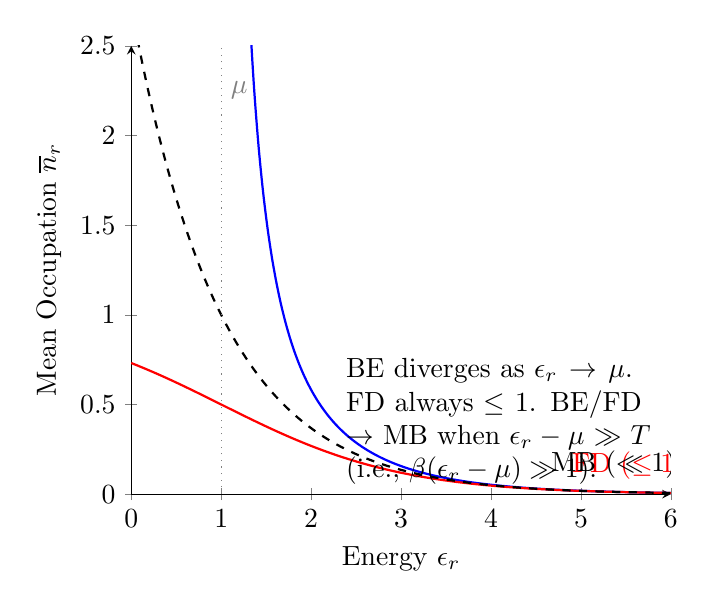
\begin{tikzpicture}
\begin{axis}[
    xlabel={Energy $\epsilon_r$}, ylabel={Mean Occupation $\overline{n}_r$},
    xmin=0, xmax=6, ymin=0, ymax=2.5,
    axis lines=left,
    legend pos=north east
]
% Assume mu = 1, beta = 1
% BE: 1/(exp(e-mu)-1)
\addplot [domain=1.01:6, samples=100, smooth, thick, blue] {1/(exp(x-1)-1)} node[pos=0.5, anchor=west] {BE};
% FD: 1/(exp(e-mu)+1)
\addplot [domain=0:6, samples=100, smooth, thick, red] {1/(exp(x-1)+1)} node[pos=0.8, anchor=south west] {FD ($\le 1$)};
% MB: exp(-(e-mu))
\addplot [domain=0:6, samples=100, smooth, thick, black, dashed] {exp(-(x-1))} node[pos=0.8, anchor=south west] {MB ($\ll 1$)};
% Mu level
\draw [gray, dotted] (axis cs:1, 0) -- (axis cs:1, 2.5) node[pos=0.9, anchor=west] {$\mu$};
\end{axis}
\node at (current axis.south east) [anchor=south east, text width=4cm] {BE diverges as $\epsilon_r \to \mu$. FD always $\le 1$. BE/FD $\to$ MB when $\epsilon_r - \mu \gg T$ (i.e., $\beta(\epsilon_r-\mu)\gg 1$).};
\end{tikzpicture}
\end{center}
Bosons (BE) have a tendency to "bunch" together at low energies ($\overline{n}_r$ can be large). Fermions (FD) obey Pauli exclusion ($\overline{n}_r \le 1$). Maxwell-Boltzmann (MB) is the low-occupation limit valid when $\eps_r - \mu \gg T$.

\section*{Single-Particle Density of States (DOS)}

Thermodynamic averages often involve sums over single-particle states $r$: $\sum_r (\dots)$.
How do we evaluate such sums?
Recall that single-particle states $\psi_r(\vec{x})$ and energies $\eps_r$ are obtained from the single-particle Schrödinger equation $H \psi_r = \eps_r \psi_r$ plus boundary conditions (BCs).

For a free particle ($H = -\frac{\hbar^2}{2m} \nabla^2$) in a large system (e.g., box of side L, volume $V=L^3$), the precise details of the BCs are usually not important for bulk properties. A convenient choice is \textbf{Periodic Boundary Conditions (PBC)}.

\textbf{1D Example:} Particle on a line of length L with PBC: $\psi(x+L) = \psi(x)$.
Schrödinger eq: $-\frac{\hbar^2}{2m} \frac{d^2\psi}{dx^2} = \eps \psi$. Solutions $\psi \sim e^{ikx}$.
Energy $\eps_k = \frac{\hbar^2 k^2}{2m}$.
PBC requires $e^{ik(x+L)} = e^{ikx} \implies e^{ikL}=1 \implies kL = 2\pi n$, where $n=0, \pm 1, \pm 2, \dots$.
Allowed wave-numbers are $k_n = \frac{2\pi n}{L}$.
Allowed energies $\eps_n = \frac{\hbar^2}{2m} (\frac{2\pi n}{L})^2 = \frac{2\pi^2\hbar^2}{mL^2} n^2$.
The sum over states $\sum_r$ becomes $\sum_{n=-\infty}^{\infty}$.
When L is large, the allowed $k$ values become closely spaced ($\Delta k = 2\pi/L$).
The number of states in a small range $dk$ is $dN_k = \frac{dk}{\Delta k} = \frac{dk}{2\pi/L} = \frac{L}{2\pi} dk$.
The sum over states can be replaced by an integral:
\[ \sum_r = \sum_n \longrightarrow \int_{-\infty}^{\infty} \frac{L}{2\pi} dk \]

\textbf{Generalization to 3D:}
Assume PBC in a box $L_x \times L_y \times L_z$. $V=L_x L_y L_z$.
Solutions $\psi(\vec{x}) \sim e^{i\vec{k}\cdot\vec{x}}$. Energy $\eps_{\vec{k}} = \frac{\hbar^2 k^2}{2m}$.
PBC requires $k_x = \frac{2\pi n_x}{L_x}$, $k_y = \frac{2\pi n_y}{L_y}$, $k_z = \frac{2\pi n_z}{L_z}$ ($n_x, n_y, n_z = 0, \pm 1, \dots$).
Allowed states form a lattice in $\vec{k}$-space.
Volume per state in $\vec{k}$-space = $(\frac{2\pi}{L_x})(\frac{2\pi}{L_y})(\frac{2\pi}{L_z}) = \frac{(2\pi)^3}{V}$.
Number of states in a small k-space volume $d^3k$: $dN_k = \frac{d^3k}{\text{Vol per state}} = \frac{V}{(2\pi)^3} d^3k$.
Sum over states becomes integral over wave-vectors:
\[ \sum_r \longrightarrow \int \frac{V}{(2\pi)^3} d^3k \]
The density of states in k-space is $\rho_{\vec{k}} = V/(2\pi)^3$.

We can now evaluate thermodynamic quantities like the grand potential:
\[ \Phi = \pm T \sum_r \ln(1 \mp e^{-\beta(\eps_r-\mu)}) \longrightarrow \Phi = \pm T V \int \frac{d^3k}{(2\pi)^3} \ln(1 \mp e^{-\beta(\eps_k-\mu)}) \]
Since $\eps_k = \hbar^2 k^2/(2m)$ depends only on $k=|\vec{k}|$, use spherical coordinates $d^3k = 4\pi k^2 dk$.
\[ \Phi = \pm T V \int_0^\infty \frac{4\pi k^2 dk}{(2\pi)^3} \ln(1 \mp e^{-\beta(\eps_k-\mu)}) = \pm \frac{TV}{2\pi^2} \int_0^\infty k^2 dk \ln(1 \mp e^{-\beta(\eps_k-\mu)}) \]

\textbf{Change variables from $k$ to $\epsilon$:} $\eps = \hbar^2 k^2/(2m)$.
$k = \sqrt{2m\eps}/\hbar \implies k^2 = 2m\eps/\hbar^2$.
$dk = \frac{\sqrt{2m}}{2\hbar} \eps^{-1/2} d\eps$.
$k^2 dk = (\frac{2m\eps}{\hbar^2}) (\frac{\sqrt{2m}}{2\hbar} \eps^{-1/2} d\eps) = \frac{m\sqrt{2m}}{\hbar^3} \sqrt{\eps} d\eps$.
\[ \Phi = \pm T \frac{V}{2\pi^2} \int_0^\infty \left( \frac{m\sqrt{2m}}{\hbar^3} \sqrt{\eps} \right) d\eps \ln(1 \mp e^{-\beta(\eps-\mu)}) \]
\[ \Phi = \pm T \int_0^\infty d\eps \, \rho(\eps) \ln(1 \mp e^{-\beta(\eps-\mu)}) \]
where $\rho(\eps)$ is the \textbf{density of states per unit energy range}:
\[ \rho(\eps) = \frac{V}{2\pi^2} \frac{m\sqrt{2m}}{\hbar^3} \sqrt{\eps} = \frac{V}{4\pi^2} \left( \frac{2m}{\hbar^2} \right)^{3/2} \sqrt{\eps} \]
$\rho(\eps) d\eps$ = number of single-particle states in the energy range $(\eps, \eps+d\eps)$.
The sum over states $\sum_r$ can be replaced by $\int d\eps \, \rho(\eps)$.

The total particle number $N$ is given by:
\[ N = \sum_r \nbar_r \longrightarrow N = \int_0^\infty d\eps \, \rho(\eps) \nbar(\eps) \]
\[ N = \int_0^\infty d\eps \, \rho(\eps) \frac{1}{e^{\beta(\eps-\mu)} \mp 1} \]
Given $N$, this integral relation determines the chemical potential $\mu = \mu(T, N, V)$.

\end{document}